%%%%%%%%%%%%%%%%%%%%%%%%%%%%%%%%%%%%%%%%%%%%%%%%%%%%%
%			ŠABLONA PÍSNIČEK v. 18.09               %
%%%%%%%%%%%%%%%%%%%%%%%%%%%%%%%%%%%%%%%%%%%%%%%%%%%%%
% Tento soubor slouží jako (naučná) šablona, pomocí 
% které lze vytvářet zdrojové soubory k jednotlivým 
% písním.
%%%%%%%%%%%%%%%%%%%%%%%%%%%%%%%%%%%%%%%%%%%%%%%%%%%%%
%			Jak psát soubory songů?                 %
%%%%%%%%%%%%%%%%%%%%%%%%%%%%%%%%%%%%%%%%%%%%%%%%%%%%%
%	1. Text písně se začíná psát na místě START 
%	   a končí na místě END. Zbylý text ignorujte.
%	2. Jak bude vypadat pdf písně zjistíte po tom, 
%	   co soubor zkompilujete pomocí souboru   
%      ../Generator/generator. 
%	3. Při psaní dodržujte následující TeX pravidla:
%	 a) Nový řádek napíšete pomocí dvou odsazení 
%	    tedy dvou enterů.
%	 b) Nová sloka se píší pomocí \sloka a odsazení.
%		Refrén se píše jako \refren, v případě více 
%		refrénů \refren[č. refrénu].
%	 c) Akordy se píšou tak, že napíšete před slovo,
%	    kde chcete mít akord (bez mezery):
%		^{AKORD1\,AKORD2...}.
%	4. Pokud chcete ušetřit tvůrcům práci, tak 
%	   si přečtěte další poučný soubor o typografii 
%	   ../../Typo_pravidla.txt.
%	5. Akordy stačí psát jen do první sloky, když 
%	   se nezmění -- kytaristé to zvládnou
%	7. Název písně pište na místo [NÁZEV] a autora 
%	   pište na místo [AUTOR] 
%	7. Jak psát věci na české klávesnici:
%	   \ = alt gr + q; [/] = alt gr f/g; 
%      {/} = alt gr + b/n; ^ = alt gr + 3 , cokoliv
%%%%%%%%%%%%%%%%%%%%%%%%%%%%%%%%%%%%%%%%%%%%%%%%%%%%%
%			Jak kompilovat jednotlivé písně?        %
%%%%%%%%%%%%%%%%%%%%%%%%%%%%%%%%%%%%%%%%%%%%%%%%%%%%%
%	1. Více návodu je k tomuto napsáno v souboru 
%      ../Generator/generator. 
%%%%%%%%%%%%%%%%%%%%%%%%%%%%%%%%%%%%%%%%%%%%%%%%%%%%%
%			Jak kompilovat celý zpěvník?			%
%%%%%%%%%%%%%%%%%%%%%%%%%%%%%%%%%%%%%%%%%%%%%%%%%%%%%
%	1. Více návodu je k tomuto napsáno v souboru
%	   ../Cely_zpevnik/zpevnik.tex.
%%%%%%%%%%%%%%%%%%%%%%%%%%%%%%%%%%%%%%%%%%%%%%%%%%%%%
\begin{song}{title=\predtitle \centering Pověste Ho Vejš \\\large Michal Tučný }  %% sem se napíše jméno songu a autor



\vspace*{.5cm}

\begin{centerjustified}

\kapodastr{2}

\vetsi
\refren Pověste ho ^{Hmi \z}vejš, ať se houpá, pověste ho ^{D \z}vejš, ať má ^{A \z}dost,

pověste ho ^{Emi \z}vejš, ať se ^{Hmi \z}houpá, že tu ^{A \z}byl nezvanej ^{Hmi \z}host.

\sloka
^{\z Hmi}Pověste ho, že byl jinej, že tu s ^{D \z}náma dejchal stejnej ^{A \z}vzduch,

^{\z Emi}pověste ho, že byl ^{Hmi \z}línej~a tak ^{\z A}trochu ^{\,\, Hmi}dobrodruh.

\sloka
^{\z Hmi}Pověste ho za El Paso, za Snídani v ^{D \z}trávě a Lodní ^{\z A}zvon,

za to, že ^{Emi \z}neoplýval ^{Hmi \z}krásou,

že měl ^{G \z}country rád a že se ^{F#7}uměl smát i ^{\z Hmi}vám.


\refren Nad ^{\z D}hlavou mi ^{A \z}slunce pálí, konec ^{Emi\z}můj~nic ^{\,\,D A}neoddálí,

do mých ^{D \z}snů se dívám ^{A \z}zdáli

a ^{Emi\z}do~uší mi stále zní ^{F#7 \z}tahle píseň poslední.

\begin{varwidth}{0.5\textwidth}
\sloka
Pověste ho za tu jistou,

který nesplnil svůj slib,

že byl zarputilým optimistou,

a tak dělal spoustu chyb.

\sloka
Pověste ho, že se koukal

a že hodně jed a hodně pil,

že dal přednost jarním loukám

a pak se oženil a pak se usadil a žil\dots

\refren 2$\times$
\end{varwidth}
\begin{varwidth}{0.3\textwidth}
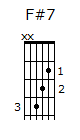
\includegraphics[width=3cm]{../Akordy/fx7}
\end{varwidth}

%Varwidth je takový boxík, který má co nejmenší velikost, ale nejméně to, co je
%napsané v nepovinném argumentu. První má velikost půlky stránky (\textwidth),
%druhá 0.3. Oba jsou vedle sebe, v jednom je text a ve druhém obrázek.
%Ty obrázky jsou ve složce akordy, když tam není žádný vhodný, musí se nový
%stáhnout z jguitar.com

\end{centerjustified}
\setcounter{Slokočet}{0}
\end{song}
